
%(BEGIN_QUESTION)
% Copyright 2012, Tony R. Kuphaldt, released under the Creative Commons Attribution License (v 1.0)
% This means you may do almost anything with this work of mine, so long as you give me proper credit

Three step-down transformers have their primary (high-voltage) terminals connected together in a ``wye'' condiguration so that the 12.5 kV line voltage energizes each primary winding with 7.2 kV.  The secondary terminals on each transformer have been left disconnected:

$$\includegraphics[width=15.5cm]{i01042x01.eps}$$

Sketch proper wire connections to provide 120/208 VAC to the customer.

\underbar{file i01042}
%(END_QUESTION)





%(BEGIN_ANSWER)

What we need here is a ``wye'' configuration on the secondary windings of the three transformers, using the center-tap of each to get 120 VAC at each phase.  The pictorial diagram shown here is one possible solution, but not the only one:

$$\includegraphics[width=15.5cm]{i01042x02.eps}$$

%(END_ANSWER)





%(BEGIN_NOTES)



%INDEX% Electronics review: 3-phase electrical power 
%INDEX% Electronics review: AC transformer circuit
%INDEX% Process: AC power distribution system (transformer)

%(END_NOTES)


